%% LR
%% Logistic Regression 逻辑回归

\subsection{LR}

% 适用场景：对连续数据进行二分分类
% 例如：利用客户的个人信息和对某商品的打分和购买情况训练模型，筛选哪一类用户会购买该商品（文本评价可通过word2vec变成连续数据、高维数据可通过PCA降维，分类结果为购买/未购买）

(a) Map xxx into a two dimensional vector space

% PCA步骤

(b) Train the model

\begin{figure}[H]
    \centering
    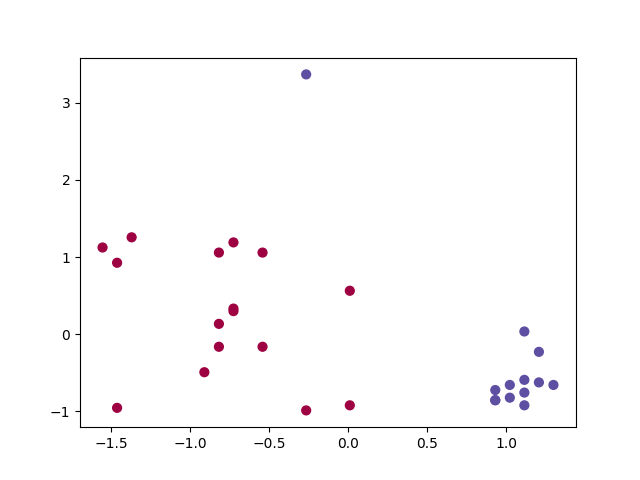
\includegraphics[width=\linewidth]{Models/clustering analysis/LR/LR_scatter.png}
    \caption{trained data}
    \label{fig:trained data}
\end{figure}

\begin{figure}[H]
    \centering
    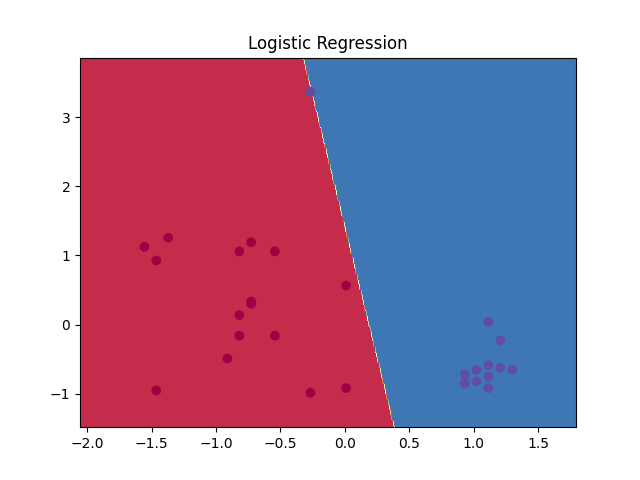
\includegraphics[width=\linewidth]{Models/clustering analysis/LR/LR.png}
    \caption{LR demo}
    \label{fig:LR_demo}
\end{figure}

(c) Predict with the model